\section{Thực nghiệm và đánh giá}\label{sec:benchmark}
\subsection{Mục tiêu và thiết lập chung}
Thực nghiệm đánh giá ba khía cạnh: tính đúng đắn, hiệu năng của hai biểu diễn
TID-set và ảnh hưởng của đặc điểm CSDL. Baseline dùng tập băm \st{};
bản tối ưu dùng vector bit \bv{} và lọc item đơn không đạt support trước khi
cấp vector. Cả hai cùng thực hiện Eclat bằng Julia; SPMF Eclat là tham chiếu
độc lập \cite{zaki,spmf}.

Bốn CSDL lấy từ FIMI \cite{fimi}, có thống kê trong Bảng~\ref{tab:data}.
Chess và Mushroom có giỏ dài; Retail có nhiều loại item nhưng giỏ ngắn;
T10I4D100K là dữ liệu tổng hợp. Giữ nguyên các giao dịch trùng nhau.
Retail và T10I4D100K được cộng 1 vào ID để đáp ứng API ID dương; phép đổi
tên này bảo toàn support. Mọi chương trình dùng cùng input đã chuẩn hóa.

\begin{table}[!ht]
\caption{Thống kê dữ liệu thực nghiệm. $N$: số giao dịch; $M$: số item;
$\bar L$: độ dài giỏ trung bình.}\label{tab:data}
\centering\small
\begin{tabular}{lrrr}\toprule CSDL & $N$ & $M$ & $\bar L$\\\midrule
Chess & 3.196 & 75 & 37,0000\\
Mushroom & 8.124 & 119 & 23,0000\\
Retail & 88.162 & 16.470 & 10,3058\\
T10I4D100K & 100.000 & 870 & 10,1023\\\bottomrule
\end{tabular}\end{table}

Với minsup tương đối $s$, ngưỡng đếm được tính theo
\begin{equation}c_{\min}=\lceil sN\rceil.\label{eq:threshold}\end{equation}
Itemset $X$ được giữ nếu số giao dịch chứa nó, $c(X)$, đạt $c_{\min}$.
Mỗi CSDL được khảo sát tại bảy ngưỡng; các ngưỡng và số đo đầy đủ nằm
trong Phụ lục~\ref{sec:appendix}.

Các lần đo ngày 16/11/2026 dùng Windows x86\_64, CPU \texttt{tigerlake}
(8 CPU logic), RAM 15,73 GiB, Julia 1.13.3 và Java 25.0.1.
Julia chạy một luồng; mỗi cấu hình được đo năm lần, báo cáo trung vị
và khoảng nhỏ nhất--lớn nhất (min--max). Cần phân biệt:
\begin{itemize}
\item \emph{Runtime toàn tiến trình}: gồm khởi động, biên dịch JIT, đọc dữ
liệu, mining và ghi kết quả; dùng để so Julia với SPMF.
\item \emph{Thời gian mining sau warm-up}: chỉ đo lần gọi \texttt{mine}
sau một lượt chạy chuẩn bị trên cùng input; dùng cho scalability và độ dài giỏ.
\item \emph{Peak RSS}: đỉnh bộ nhớ thường trú của tiến trình đến hết mining,
không phải tổng lượng cấp phát hay bộ nhớ riêng của thuật toán.
\end{itemize}
Các chương trình chạy tuần tự, luân phiên thứ tự. Đối chiếu correctness
nằm ngoài phần đo. Chi tiết warm-up, GC và checksum được đưa vào
Phụ lục~\ref{sec:appendix} để tách khỏi phần đọc kết quả.

\subsection{Kiểm tra tính đúng đắn}
Mục tiêu là xác nhận hai backend trả về đúng tất cả itemsets và support count.
Output được chuẩn hóa thành ánh xạ itemset--số đếm rồi so sánh với SPMF.
Một cấu hình đạt khi không thiếu itemset, không thừa itemset và không sai support.

Bảng~\ref{tab:correct} cho thấy cả hai backend khớp 100\% trên năm CSDL đầy đủ:
bốn benchmark và Groceries. Ngoài đối chiếu này, bộ test Julia có 439/439
assertions đạt, bao gồm các trường hợp biên, I/O và luật kết hợp.
Toàn bộ 560 mẫu hiệu năng đã lưu cũng khớp tham chiếu SPMF.

\begin{table}[!ht]\caption{Correctness trên CSDL đầy đủ. Set và BitVector đều khớp SPMF 100\% ở mọi dòng.}\label{tab:correct}\centering\small
\begin{tabular}{lrrr}\toprule CSDL & $N$ & $s$ (\%) & Itemsets\\\midrule
Groceries & 9.835 & 1 & 333\\ Chess & 3.196 & 87,5 & 1.386\\
Mushroom & 8.124 & 70 & 31\\ Retail & 88.162 & 4 & 18\\
T10I4D100K & 100.000 & 1,5 & 237\\\bottomrule\end{tabular}\end{table}

\subsection{Runtime và số itemset theo minsup}
\textbf{Thiết lập.} Với mỗi CSDL, giảm minsup qua bảy mức và đo Set,
BitVector, SPMF trong cùng đợt. Có $4\times7\times3\times5=420$ mẫu runtime.
Hình~\ref{fig:runtime} biểu diễn thời gian toàn tiến trình;
Hình~\ref{fig:counts} biểu diễn số itemsets tương ứng.

\textbf{Kết quả.} BitVector có trung vị thấp hơn Set ở 23/28 cấu hình;
SPMF thấp hơn cả hai ở 28/28 cấu hình. Tại ngưỡng thấp nhất của Retail,
Chess, Mushroom và T10I4D100K, tỷ số $t_{Set}/t_{BV}$ lần lượt là
1,16; 1,59; 1,20; 2,24. Lợi ích không đồng đều: ở Retail 4\%,
BitVector mất 2,2609 s, cao hơn Set 2,1022 s.

\textbf{Giải thích.} Khi giảm minsup, số itemsets tăng hoặc giữ nguyên.
Chess tăng từ 77 lên 8.227 itemsets khi minsup giảm từ 95\% xuống 80\%;
Mushroom tăng từ 7 lên 565 trong dải ngưỡng khảo sát. Retail và T10I4D100K
ở ngưỡng thấp nhất lần lượt có 580 và 1.073 itemsets. Vì vậy số giao dịch
lớn hơn không nhất thiết tạo nhiều kết quả hơn; phân bố đồng xuất hiện
và minsup quyết định số tổ hợp đạt ngưỡng.

Eclat mở rộng nhánh bằng giao các tập mã giao dịch:
$T(X\cup Y)=T(X)\cap T(Y)$ \cite{zaki}.
Nhiều tổ hợp đạt support tạo thêm phép giao, nhánh DFS và kết quả cần lưu.
Thời gian thực tế còn bao gồm khởi động/JIT và I/O, nên không bắt buộc tăng
ở từng điểm. SPMF nhanh hơn trong phạm vi toàn tiến trình đã đo; chưa thể
từ đó suy ra riêng tốc độ phần mining của hai ngôn ngữ.

\begin{reportfigure}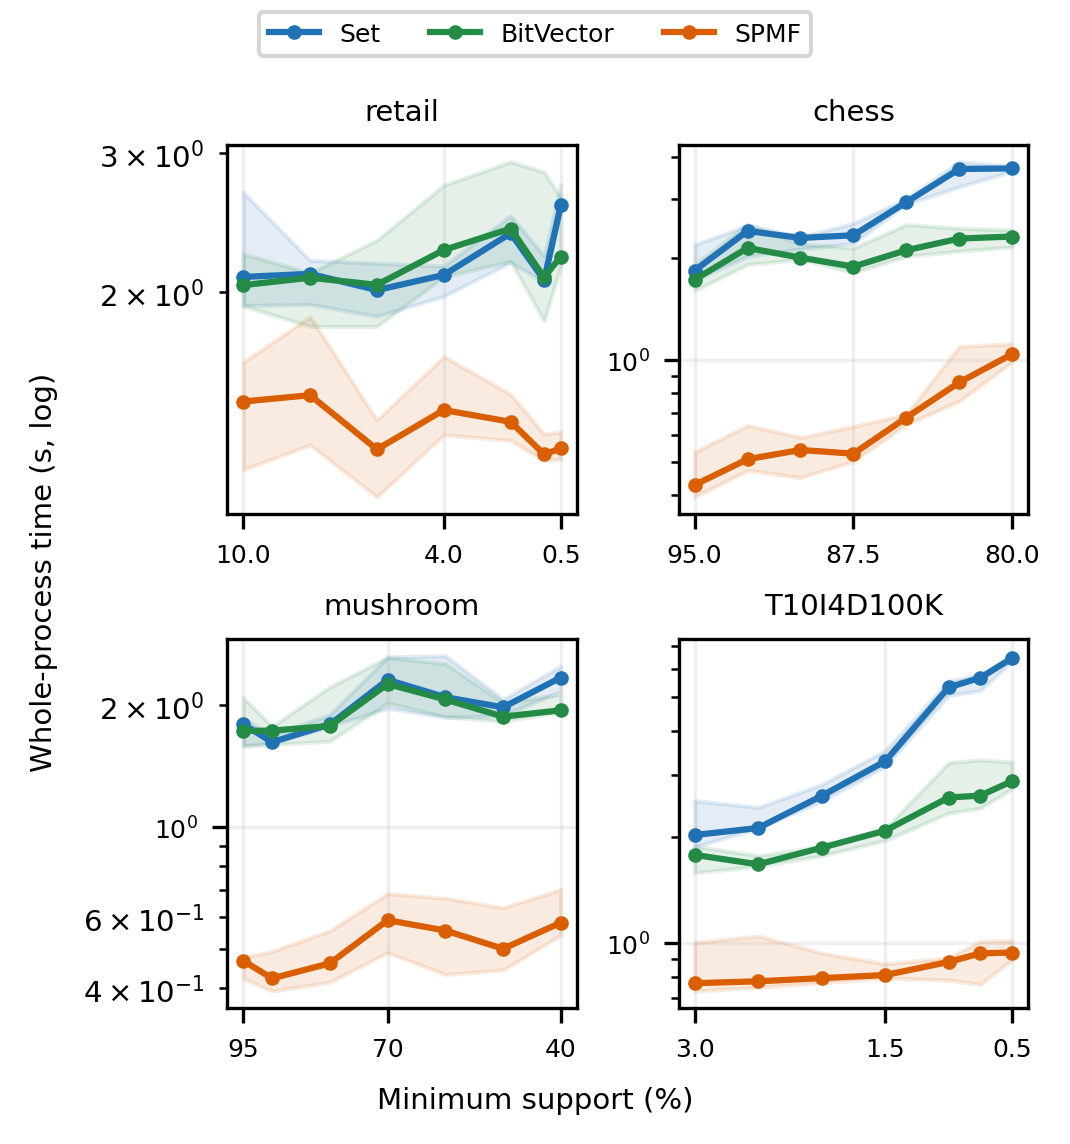
\includegraphics[width=\columnwidth]{runtime.png}
\caption{Runtime toàn tiến trình theo minsup giảm dần: trung vị năm lần và vùng min--max; trục thời gian dùng thang log.}\label{fig:runtime}\end{reportfigure}
\begin{reportfigure}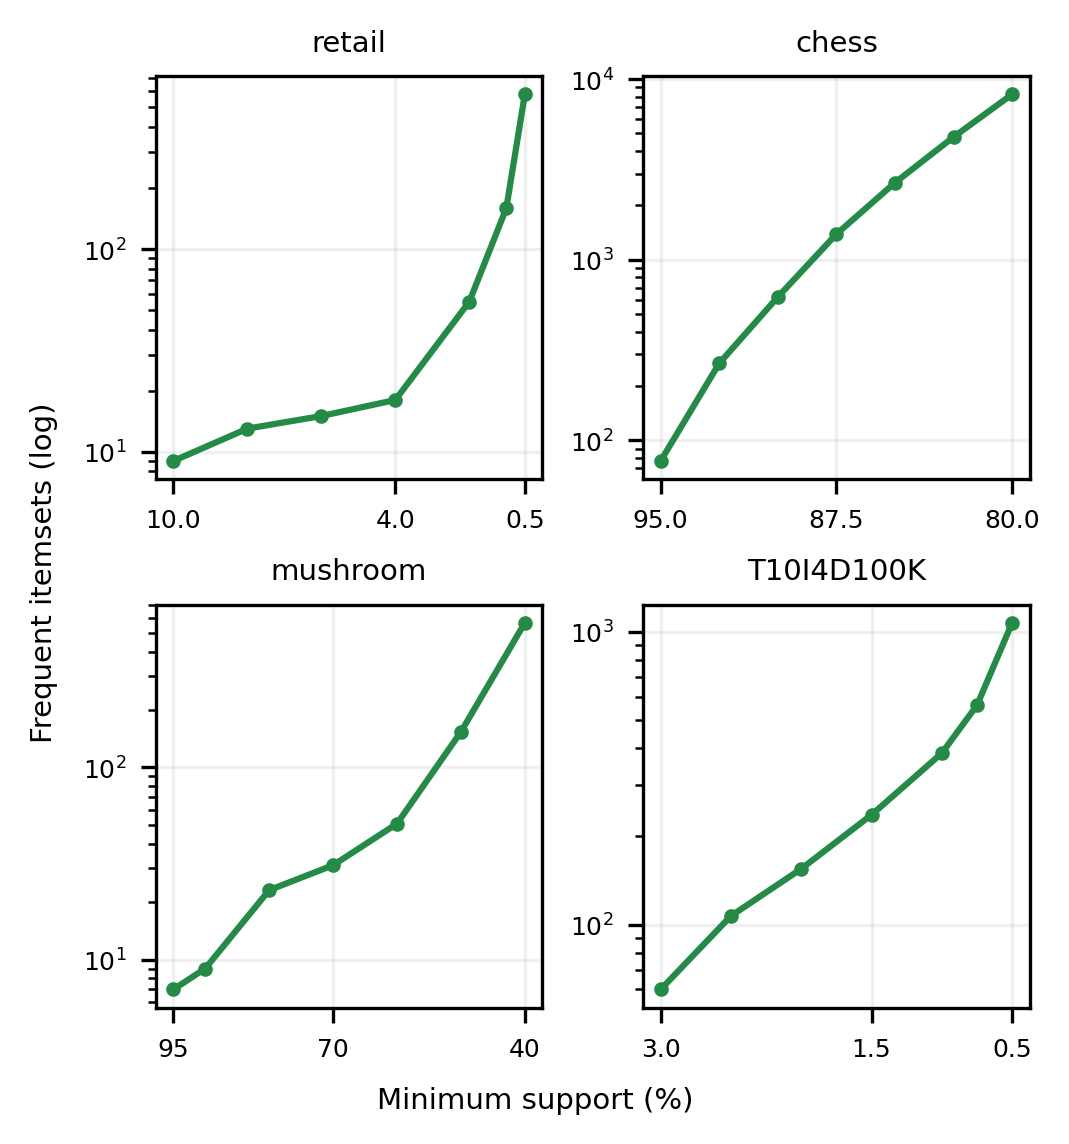
\includegraphics[width=\columnwidth]{counts.png}
\caption{Số itemsets theo minsup; Set, BitVector và SPMF khớp chính xác cả itemset và support ở mọi cấu hình.}\label{fig:counts}\end{reportfigure}

\subsection{Peak RAM: baseline so với optimized}
\textbf{Thiết lập.} Đo mỗi backend trong năm tiến trình riêng tại điểm thứ
tư của dải bảy minsup: Retail 4\%, Chess 87,5\%, Mushroom 70\%,
T10I4D100K 1,5\%. Peak RSS được lấy ngay sau mining, trước khi ghi output.

\textbf{Kết quả.} Bảng~\ref{tab:ram} và Hình~\ref{fig:ram} cho thấy BitVector
giảm median Peak RSS 2,15--10,27\%; Retail giảm nhiều nhất.
Mức giảm được tính bằng
\begin{equation}\Delta_M=100\left(1-\frac{\widetilde M_{BV}}{\widetilde M_{Set}}\right),\end{equation}
với $\widetilde M$ là trung vị Peak RSS của năm tiến trình, tính bằng MiB.

\begin{reporttable}
\caption{Peak RSS tại minsup trung bình: median năm tiến trình, đơn vị MiB; mức giảm tính từ median.}\label{tab:ram}
\centering\footnotesize
\begin{tabular}{lrrrr}\toprule
CSDL & $s$ (\%) & Set & BV & Giảm (\%) \\\midrule
retail & 4,0 & 268,98 & 241,36 & 10,27 \\
chess & 87,5 & 245,35 & 228,95 & 6,69 \\
mushroom & 70,0 & 232,04 & 227,05 & 2,15 \\
T10I4D100K & 1,5 & 289,16 & 266,75 & 7,75 \\
\bottomrule\end{tabular}
\end{reporttable}
\begin{reportfigure}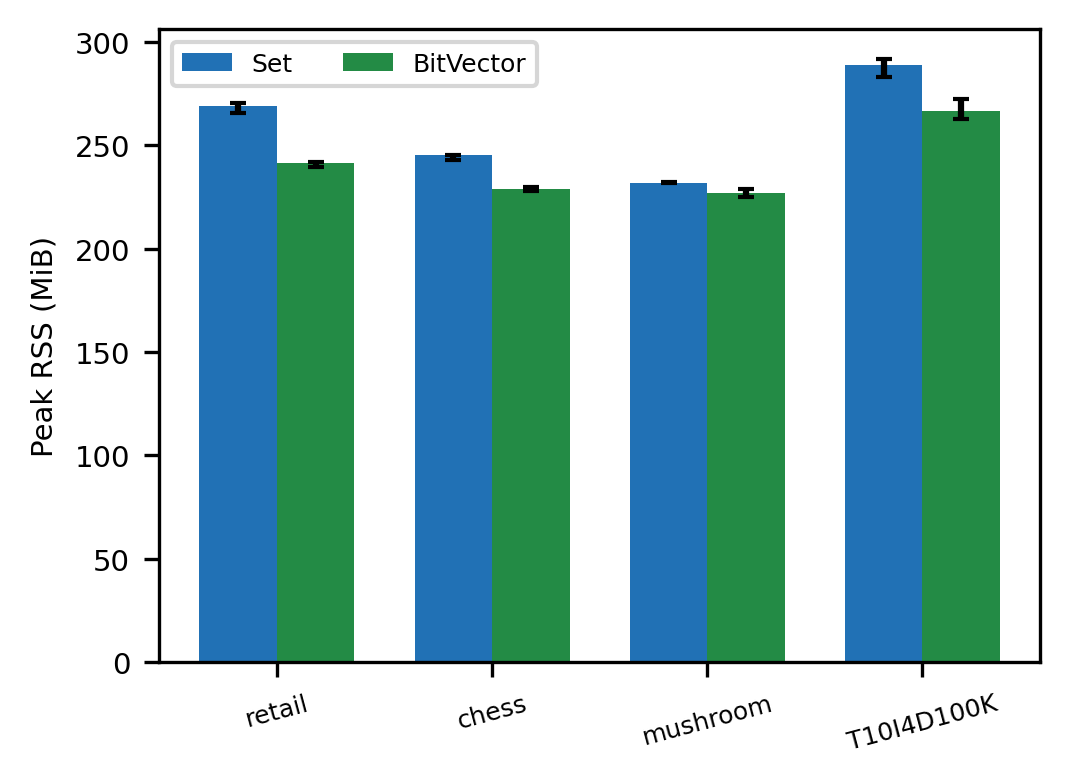
\includegraphics[width=\columnwidth]{ram.png}
\caption{Peak RSS tại minsup trung bình; thanh sai số là min--max của năm tiến trình.}\label{fig:ram}\end{reportfigure}

\textbf{Giải thích.} Mỗi BitVector cần xấp xỉ $N$ bit, chưa tính overhead.
Nếu cấp vector cho mọi item trước khi lọc, nhiều item hiếm vẫn chiếm
vector đầy đủ. Bản hiện tại đếm support trước, chỉ cấp vector cho item đạt
ngưỡng rồi quét lại input để bật bit. Ở Retail 4\%, chỉ 7/16.470 item sống
sót, nên tránh được nhiều vector không cần thiết.

Set chỉ lưu TID có mặt nhưng có chi phí bảng băm. BitVector lưu gọn hơn
khi tập TID đủ dày; lợi ích còn phụ thuộc số item được giữ. Các số RSS trên
bao gồm cả runtime, input và output, nên không được diễn giải là mức giảm
riêng của cấu trúc TID-set.

\subsection{Khả năng mở rộng theo số giao dịch}
\textbf{Thiết lập.} Chọn các tập con Retail 10\%, 25\%, 50\%, 75\%, 100\%
từ một hoán vị chỉ số có seed cố định. Các tập con lồng nhau; mức 100\%
chính là 88.162 giao dịch ban đầu. Đây là tăng số giao dịch được chọn,
không nhân bản CSDL. Giữ minsup 4\% và đo \texttt{mine} sau warm-up.

\textbf{Kết quả.} Theo Bảng~\ref{tab:scale} và Hình~\ref{fig:scale}, khi N
tăng xấp xỉ 10 lần, trung vị thời gian Set tăng 14,028 lần, BitVector
tăng 9,554 lần. Tại toàn bộ Retail, Set mất 105,122 ms còn BitVector
39,658 ms, tức BitVector nhanh hơn khoảng 2,65 lần. Cả năm mức có 18 itemsets.

\begin{reporttable}
\caption{Scalability Retail: thời gian mine sau warm-up, median năm lần (ms); mọi mức có 18 itemsets.}\label{tab:scale}
\centering\footnotesize
\begin{tabular}{rrrrr}\toprule
Tỷ lệ (\%) & $N$ & $c_{\min}$ & Set (ms) & BV (ms) \\\midrule
10 & 8816 & 353 & 7,494 & 4,151 \\
25 & 22040 & 882 & 24,107 & 11,557 \\
50 & 44081 & 1764 & 51,274 & 21,116 \\
75 & 66121 & 2645 & 81,147 & 29,829 \\
100 & 88162 & 3527 & 105,122 & 39,658 \\
\bottomrule\end{tabular}
\end{reporttable}
\begin{reportfigure}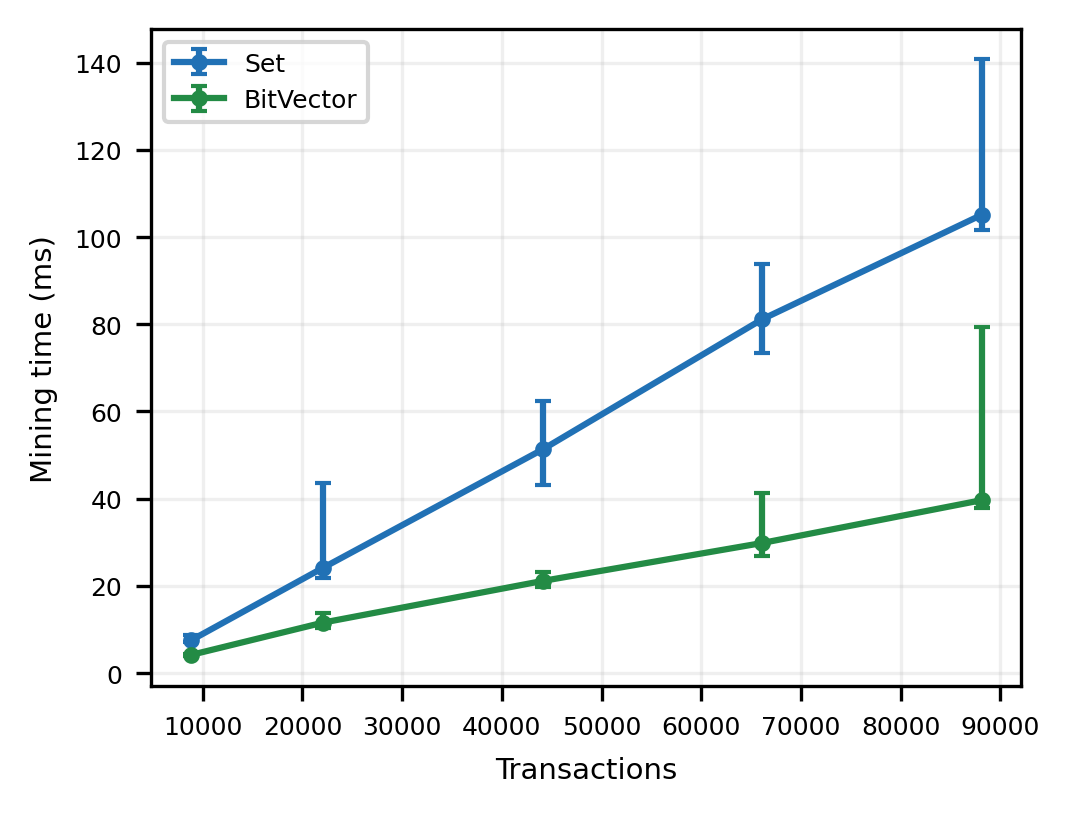
\includegraphics[width=\columnwidth]{scale.png}
\caption{Scalability Retail tại minsup 4\%: trung vị thời gian mining sau warm-up và khoảng min--max.}\label{fig:scale}\end{reportfigure}

\textbf{Giải thích.} Tập giao dịch lớn hơn làm các tập TID hoặc vector bit
lớn hơn, tăng chi phí dựng và giao tập. Trong miền đo này, thời gian tăng
gần tuyến tính theo N. Khớp mô tả $t=aN+b$ trên năm trung vị có
$R^2=0,9990$ với Set và $0,9977$ với BitVector.
Tuy nhiên, năm điểm có output ổn định không chứng minh Eclat có độ phức
tạp tuyến tính tổng quát; số ứng viên và nhánh có thể thay đổi khi đổi minsup.

\subsection{Ảnh hưởng độ dài giao dịch trung bình}
\textbf{Thiết lập.} Giữ $N=5.000$, $M=64$, minsup 5\% và $c_{\min}=250$;
tăng độ dài mỗi giỏ qua $L=4,8,12,16,20$. Mỗi TID có một hoán vị item riêng;
mức L lấy L item đầu của cùng hoán vị. Giỏ dài chứa toàn bộ item của giỏ
ngắn tương ứng, nên support của itemset cũ không giảm. Mọi mức đều quan sát
đủ 64 item và được đo mining sau warm-up.

\textbf{Kết quả.} Bảng~\ref{tab:length} và Hình~\ref{fig:length} cho thấy L
tăng 5 lần làm thời gian Set tăng 55,311 lần, BitVector tăng 10,909 lần.
Bước từ L=12 sang L=16 làm số itemsets tăng mạnh từ 64 lên 2.077.
Ở L=20, tỷ số thời gian Set/BitVector là 93,54; tỷ số này thuộc phép đo
mining sau warm-up, khác phép đo toàn tiến trình ở trên.

\begin{reporttable}
\caption{Độ dài giao dịch: median năm lần sau warm-up (ms); N=5.000, M=64 và minsup 5\%.}\label{tab:length}
\centering\footnotesize
\begin{tabular}{rrrrr}\toprule
$L$ & Mật độ (\%) & Itemsets & Set (ms) & BV (ms) \\\midrule
4 & 6,25 & 64 & 14,541 & 0,788 \\
8 & 12,50 & 64 & 33,975 & 1,486 \\
12 & 18,75 & 64 & 60,846 & 2,053 \\
16 & 25,00 & 2077 & 485,904 & 8,747 \\
20 & 31,25 & 2080 & 804,295 & 8,598 \\
\bottomrule\end{tabular}
\end{reporttable}
\begin{reportfigure}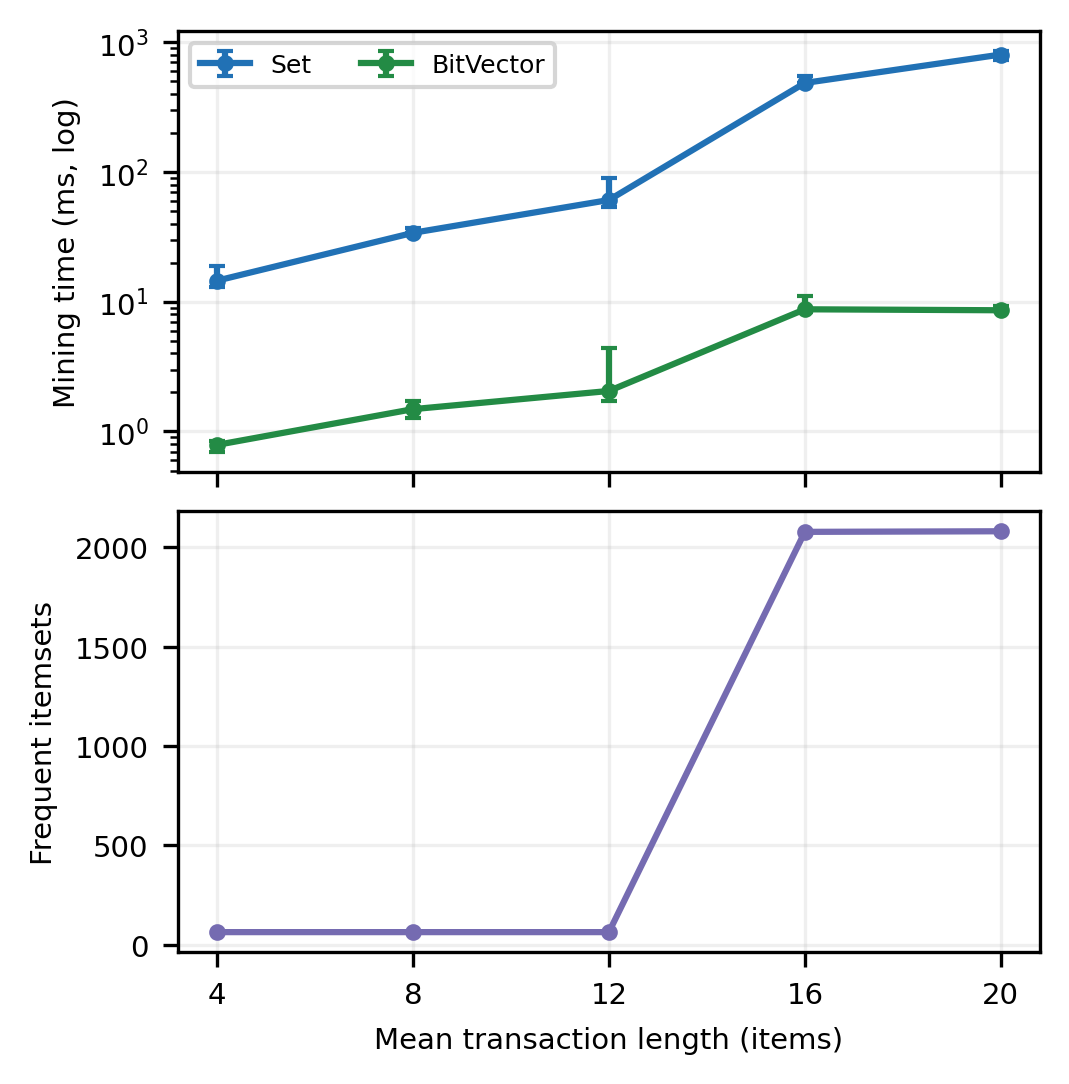
\includegraphics[width=\columnwidth]{length.png}
\caption{Thời gian mining sau warm-up và output size khi tăng độ dài giỏ; N, M và minsup cố định. Trục thời gian dùng thang log.}\label{fig:length}\end{reportfigure}

\textbf{Giải thích.} Giỏ dài hơn làm nhiều item cùng xuất hiện hơn, tạo
TID-set dày hơn và nhiều tổ hợp đạt support hơn. Với chọn đều L item từ M,
xác suất một cặp cụ thể xuất hiện là
\begin{equation}p_2=\frac{L(L-1)}{M(M-1)}.\end{equation}
Support cặp kỳ vọng $Np_2$ tăng từ khoảng 163,7 tại L=12 lên 297,6 tại
L=16, vượt ngưỡng 250. Điều này giải thích vì sao output có thể tăng
mạnh ở bước đó. Set phải xử lý nhiều TID; BitVector giữ chiều dài theo N
nhưng vẫn phải giao thêm ứng viên và lưu thêm kết quả.

\subsection{Giới hạn và hướng tối ưu tiếp}
Các phép đo dùng một máy, năm lần lặp và một seed cho mỗi thiết kế ngẫu
nhiên. Khoảng min--max là dao động quan sát, không phải khoảng tin cậy.
Chưa tách riêng đóng góp của JIT, GC, I/O và cache. Vì vậy các kết luận
áp dụng cho cấu hình đã đo; không trộn thời gian toàn tiến trình với thời
gian mining sau warm-up hoặc coi Peak RSS là bộ nhớ riêng thuật toán.
Eclat còn phụ thuộc số tổ hợp ứng viên và kích thước output, có thể tăng
theo hàm mũ của số item.

Hai hướng tiếp theo là: (1) chọn biểu diễn TID theo mật độ, dùng cấu trúc
thưa cho tập ít TID và bitset cho tập dày; (2) giảm cấp phát khi giao
BitVector, chẳng hạn đếm giao trước hoặc tái sử dụng bộ đệm riêng cho từng
mức DFS. Khi đánh giá, cần tính cả chi phí chuyển biểu diễn và kiểm tra
itemset/support trước khi kết luận có cải thiện. Đây là đề xuất chưa được
đo trong báo cáo.

% Render at the end of the report, after the bibliography.
\newcommand{\EclatBenchmarkAppendix}{%
\appendices
\section{Chi tiết tái lập và số đo}\label{sec:appendix}
Phụ lục này lưu thông tin kỹ thuật bổ trợ cho Chương II.
Seed dùng cho chọn tập con Retail và sinh giỏ tổng hợp là 20261116,
bộ sinh \texttt{MersenneTwister}. Mỗi TID có hoán vị item riêng khi sinh
giỏ; các mức L dùng tiền tố của cùng hoán vị. Tập con Retail được lấy
từ tiền tố hoán vị chỉ số dòng, sau đó sắp theo thứ tự dòng gốc.

Trong phép đo toàn tiến trình, mỗi cấu hình có một lượt chuẩn bị không
ghi nhận cho mỗi chương trình; năm lượt ghi nhận vẫn là tiến trình mới
và vẫn tính JIT. Chuẩn hóa input, mở log và so sánh output nằm ngoài đồng hồ.
Trong hai phép đo mining, tiến trình đọc input, warm-up một lần trên đúng
CSDL/cùng minsup, gọi bộ gom rác (GC), rồi đo một lần \texttt{mine}.
GC bên trong mining được tính; các bước trước đo và ghi output không được tính.

Peak RSS lấy bằng \texttt{Sys.maxrss()} ngay sau mining; trên Windows đây
là peak working set \cite{windowsrss}. Warm-up trên cùng một CSDL nhỏ,
GC, đọc input thật rồi GC trước mining. Đỉnh toàn tiến trình không reset
sau warm-up, nên không trừ đỉnh trước mining để gọi phần chênh là RAM riêng
thuật toán. MiB bằng $2^{20}$ byte.

Dữ liệu gốc, input chuẩn hóa, JAR và source được nhận diện bằng SHA-256
trong metadata của từng thí nghiệm. JAR SPMF không được suy phiên bản từ
nhãn thuật toán trong log. Các CSV \texttt{runs.csv} lưu từng mẫu,
\texttt{summary.csv} lưu median/min/max; metadata ghi môi trường và cách đo.
Có 420 mẫu runtime, 40 mẫu RAM, 50 mẫu scalability và 50 mẫu độ dài giỏ.

Bảng~\ref{tab:runtime} giữ toàn bộ 28 cấu hình runtime theo bảy minsup của
từng CSDL. Cả hai backend đều khớp SPMF ở mọi cấu hình.
\begin{reporttable}
\caption{Toàn bộ cấu hình runtime. Thời gian là median năm lần, đơn vị giây; BV là BitVector. Tất cả cấu hình khớp SPMF.}\label{tab:runtime}
\centering\footnotesize
\begin{tabular}{lrrrrrr}\toprule
CSDL & $s$ (\%) & Itemsets & Set (s) & BV (s) & SPMF (s) & Set/BV \\\midrule
retail & 10,00 & 9 & 2,0903 & 2,0409 & 1,4530 & 1,02 \\
retail & 8,00 & 13 & 2,1091 & 2,0854 & 1,4801 & 1,01 \\
retail & 6,00 & 15 & 2,0114 & 2,0429 & 1,2637 & 0,98 \\
retail & 4,00 & 18 & 2,1022 & 2,2609 & 1,4174 & 0,93 \\
retail & 2,00 & 55 & 2,3744 & 2,4071 & 1,3694 & 0,99 \\
retail & 1,00 & 159 & 2,0704 & 2,0881 & 1,2454 & 0,99 \\
retail & 0,50 & 580 & 2,5762 & 2,2182 & 1,2675 & 1,16 \\
chess & 95,00 & 77 & 1,8420 & 1,7313 & 0,4285 & 1,06 \\
chess & 92,50 & 267 & 2,4119 & 2,1480 & 0,5105 & 1,12 \\
chess & 90,00 & 622 & 2,2990 & 2,0107 & 0,5436 & 1,14 \\
chess & 87,50 & 1386 & 2,3415 & 1,8924 & 0,5300 & 1,24 \\
chess & 85,00 & 2669 & 2,9334 & 2,1150 & 0,6775 & 1,39 \\
chess & 82,50 & 4777 & 3,6756 & 2,2894 & 0,8610 & 1,61 \\
chess & 80,00 & 8227 & 3,6887 & 2,3216 & 1,0436 & 1,59 \\
mushroom & 95,00 & 7 & 1,7943 & 1,7274 & 0,4677 & 1,04 \\
mushroom & 90,00 & 9 & 1,6213 & 1,7304 & 0,4234 & 0,94 \\
mushroom & 80,00 & 23 & 1,7923 & 1,7772 & 0,4611 & 1,01 \\
mushroom & 70,00 & 31 & 2,3096 & 2,2552 & 0,5892 & 1,02 \\
mushroom & 60,00 & 51 & 2,0924 & 2,0652 & 0,5557 & 1,01 \\
mushroom & 50,00 & 153 & 1,9754 & 1,8734 & 0,5009 & 1,05 \\
mushroom & 40,00 & 565 & 2,3397 & 1,9420 & 0,5811 & 1,20 \\
T10I4D100K & 3,00 & 60 & 2,0288 & 1,7810 & 0,7692 & 1,14 \\
T10I4D100K & 2,50 & 107 & 2,1238 & 1,6746 & 0,7787 & 1,27 \\
T10I4D100K & 2,00 & 155 & 2,6211 & 1,8671 & 0,7950 & 1,40 \\
T10I4D100K & 1,50 & 237 & 3,2873 & 2,0871 & 0,8115 & 1,58 \\
T10I4D100K & 1,00 & 385 & 5,3349 & 2,5934 & 0,8840 & 2,06 \\
T10I4D100K & 0,75 & 561 & 5,6774 & 2,6263 & 0,9353 & 2,16 \\
T10I4D100K & 0,50 & 1073 & 6,4633 & 2,8884 & 0,9402 & 2,24 \\
\bottomrule\end{tabular}
\end{reporttable}
}
